\chapter{$z$-Transform}

In mathematics and signal processing, the $z$-Transform converts a discrete-time signal, which is a sequence of real or complex numbers, into a complex frequency-domain (z-domain or z-plane) representation.

It can be considered as a discrete-time equivalent of the Laplace transform (s-domain).

Whereas the continuous-time Fourier transform is evaluated on the Laplace s-domain's imaginary line, the discrete-time Fourier transform is evaluated over the unit circle of the z-domain. What is roughly the s-domain's left half-plane, is now the inside of the complex unit circle; what is the z-domain's outside of the unit circle, roughly corresponds to the right half-plane of the s-domain.

One of the means of designing digital filters is to take analog designs, subject them to a bilinear transform which maps them from the s-domain to the z-domain, and then produce the digital filter by inspection, manipulation, or numerical approximation. Such methods tend not to be accurate except in the vicinity of the complex unity, i.e. at low fre\-quen\-cies\cite{bib:zTransform}.

The Discrete-time Fourier Transform provides a frequency-domain representation of discrete-time signals and LTI dis\-cre\-te-time systems. Because of the convergence condition as in Equation~\ref{thm:existenceDTFT}, in many cases the DTFT of a sequence might not exist. As a consequence, it is not possible to make use of such frequency characterization in all cases where the transform does not converge.

A generalization of the Discrete-time Fourier Transform is the
\textbf{$z$-Transform}, defined by
\begin{equation}\label{eqn:zTransform}
    G(z) = \sum_{n=-\infty}^\infty g[n] z^{-n},
\end{equation}
where the \emph{$z$-frequency} $z := \Re{(z)} + j \Im{(z)}$ is a complex
variable.

If one lets $z = re^{j\omega}$, it is straightforward to notice that the
$z$-transform reduces to
\begin{equation}\label{eqn:zTransformInterpretation}
    G(re^{j\omega}) = \sum_{n=-\infty}^\infty g[n] r^{-n} e^{-j\omega n},
\end{equation}
and given that the formula for the Discrete-time Fourier Transform is
\[
    X(e^{j\omega}) = \sum_{n=-\infty}^\infty x[n]e^{-j\omega n}
\]
one concludes that $G(re^{j\omega})$ can be interpreted as the DTFT of the modified sequence $\{g[n]r^{-n}\}$. For $r = 1$ one has $|z| = 1$, and the $z$-transform reduces to its DTFT, provided the latter exists. For sure, the $z$-transform is decisive in all case where a DTFT of a sequence does not exist, hence when the sequece is not suitable to be transformed into Fourier domain.

Since a $z$-transform of a sequence $g[n]$ with $r = 1$ is completely equivalent to a DTFT of the same input sequence, the DTFT reduces to compute the $z$-transform and evaluating it at $z$-frequencies such that $|z| = 1$; this practically means that amid all possible complex frequencies, the DTFT is like evaluating the $z$-transform in the \textbf{unit circle} of radius $1$, that is the countour $|z| = 1$. The complex variable $z = re^{j\omega}$ can be split into two components, $r$ and a complex exponential $e^{j\omega}$. The first term is the \emph{distance between the point and the origin} in the z-plane (the radius), the second one determines the \emph{angle} at which the complex number is located. When $r=1$, we are basically lying in the contour of the unit circle as $z$ will possess module $|z|=1$. At last, the $z$-transform is an extension of the Discrete-time Fourier Transform, from the circle of radius $1$ to all complex domain.

\section{Properties of $z$-Transform}

\subsection{Region of Convergence}

Like the DTFT, there are conditions on the convergence of the infinite series in the definition~\ref{eqn:zTransform}; for a given sequence the set $\mathcal R$ of the values of $z$ among which the $z$-transform converges is said to be the \textbf{region of convergence (RoC)} of the $z$-transform.

In particular due to Theorem~\ref{thm:existenceDTFT}, the series
\[
    G(re^{j\omega}) = \sum_{n=-\infty}^\infty g[n] r^{-n} e^{-j\omega n}
\]
converges if the sequence $\{g[n]r^{-n}\}$ is absolutely summable, that is when
\[
    \sum_{n=-\infty}^\infty \left|g[n] r^{-n}\right| < \infty.
\]

The $z$-transform may converge only in a specific region of the z-plane, precisely the RoC. Let $r_-=\mathcal R_{g-}$ and $r_+ = \mathcal R_{g+}$ be the values of $r$ among which the $z$-transform converges; then, the sequence $g[n]r^{-n}$ is \emph{absolutely summable} for all such values of $r$, that is
\[
    \sum_{n=-\infty}^\infty \left|g[n] r^{-n}\right| < \infty
\]
in the range \[ 0 \leq r_- \leq r \leq r_+ \leq \infty.\] The annular region defined by the previous inequalities is called the \emph{region of convergence (RoC)} of $G(re^{j\omega}) = G(z)$, and can be geometrically illustrated as in the next Figure,

\begin{center}
    \begin{tikzpicture}
        \draw[thick,-stealth] (-2.5,0) -- (2.5,0) node[anchor=north west] {$\Re z$};
        \draw[thick,-stealth] (0,-2.5) -- (0,2.5) node[anchor=south east] {$\Im z$};
        \node[draw, circle, minimum size=4cm] at (0,0){};
        \node[draw, circle, minimum size=3cm] at (0,0){};
        \draw[-stealth] (0,0) -- (2*0.7071, 2*0.7071);
        \draw[-stealth] (0,0) -- (-1.5000*0.7071, 1.5000*0.7071);
        \node[] at (+2.3*0.7, 2.3*0.7) {$\mathcal{R}_{g+}$};
        \node[] at (-0.8*0.7, 1.5*0.7) {$\mathcal{R}_{g-}$};
        \node[] at (-3, 1) {RoC};
        \draw[-stealth, dashed] (-2.65,1) .. controls (-1.85,1) and (-1.5,1.7) .. (-0.5,1.7);
        \path[pattern=north east lines, pattern color=blue, opacity=.5, even odd rule]
            (-3, -3) rectangle (3,3)
            (-3, -3) rectangle (3,3)
            (0,0) circle[radius=1.5]
            (0,0) circle[radius=2];
    \end{tikzpicture}
\end{center}

A decisive remark is that a $z$-transform \emph{should always be accompanied by the relative region of convergence}. As a matter of fact, it is entirely meaningless to define a $z$-transform without its RoC, since the latter is a crucial information.

As an example, let's determine the $z$-transform $X(z)$ of a causal exponential sequence $x[n] = \alpha^n \mu[n]$, along with its region of convergence. To do so, compute
\begin{align*}
    X(z) &= \sum_{n=-\infty}^\infty \alpha^n \mu[n] z^{-n} = \sum_{n=0}^\infty \alpha^n z^{-n}\\
         &= \frac{1}{1 - \alpha z^{-1}}.
\end{align*}
Now, the region of convergence---the above power series converges to the above fraction only if $\left|\alpha z^{-1}\right| < 1$, which yields an annular region of convergence of $|z| > |\alpha|$. Aforesaid region is where the $z$-transform lives, since there the series is absolutely summable in all values.

It immediately follows that, by picking $\alpha = 1$, the $z$-transform of the sequence $x[n] = \mu[n]$ will be
\[
    X(z) = \frac {1} {1 - z^{-1}}, \mbox{ for } \left|z^{-1}\right| < 1
\]
with a RoC of $\infty \geq |z| > 1$. Indeed, this is akin to the previous case, but with $\alpha = 1$.

Remarkably, notice that the unit step sequence $\mu[n]$ is not absolutely summable. This is consistent with the obtained results: its $z$-transform is characterized by a region of convergence of $|z| > 1$; the Discrete-time Fourier Transform exists on the unit circle $|z| = 1$, and in order for it to exist and ultimately converge uniformly the region of convergence of the $z$-transform should have included the unit circle, which is not the case for the unit step sequence.

Evaluate now the anti-causal sequence
\[
    y[n] = -\alpha^n \mu[-n-1]
\]
which is very consonant with the previously-analyzed sequence $x[n] = \alpha^n
\mu[n]$. Its $z$-transform is
\begin{align*}
    Y(z)
    &= \sum_{n=-\infty}^{\infty} -\alpha^n z^{-n} = -\sum_{n=-\infty}^{-1} \alpha^n z^{-n} =\\
    &= -\sum_{m=1}^{\infty} \alpha^{-m} z^{m} = -\alpha^{-1}z \sum_{m=0}^{\infty} -\alpha^{-m} z^{m} =\\
    &= \frac{\alpha^{-1}z}{1 - \alpha^{-1}z} = \frac{1}{1 - \alpha z^{-1}}, \mbox{ for } \left|\alpha^{-1} z\right| < 1
\end{align*}
yielding a RoC of $|z| < |\alpha|$, which is quite the opposite of the previous case; this region of convergence is related to an anti-causal signal in place of a causal signal.

Please take a moment to consider that the $z$-transforms of the two sequences $\alpha^n \mu[n]$ and $-\alpha^n\mu[-n-1]$ are \emph{identical}, even though the two parent sequences are different: what in reality differs, are the two regions of convergence. This is the exact reason why it is paramount to first determine and then specify the RoC for each and every $z$-transform one has to manipulate.

All the convergence considerations we have hitherto ex\-pres\-sed culminate in the following theorem, which states the conditions under which a DTFT converges uniformly in terms of the characteristics that the region of convergence of its $z$-transform possesses.

\begin{thm}[Uniform convergence of the DTFT]\label{thm:convergenceDTFTz}
    Let $G(e^{j\omega})$ be a Discrete-time Fourier Transform of a sequence $g[n]$. $G$ \emph{converges uniformly} if and only if the Region Of Convergence of the $z$-transform $G(z)$ of $g[n]$ includes the unit circle, that is if and only if it includes $|z| = 1$.
\end{thm}

Moreover, the existence of the DTFT does not always imply the existence of the $z$-transform, since the first exists only in terms of \emph{mean square convergence}, or it has impulses. Very much, the following example illustrates this apparent paradox: let the finite energy sequence
\[
    h_{LP}[n] = \frac{\sin{\omega_c n}}{\pi n}, -\infty < n < \infty
\]
be. Its DTFT is the following function,
\[
    H_{LP}(e^{j\omega}) = 
    \left\{
        \begin{array}{ll}
            1 & 0 \leq |\omega| \leq \omega_c\\
            0 & \omega_c < |\omega| \leq \pi
        \end{array}
    \right.
\]
which converges in the mean-square sense. However, $h_{LP}[n]$ does not possess a $z$-transform, and it is not absolutely sum\-ma\-ble for any value of $r$ when performing the $z$-transform! Basically, it might happen that despite a DTFT exists, a $z$-transform does not. The following Table~\ref{tab:zTransforms} illustrates some of the most commonly used $z$-transform pairs.

\begin{table}[ht]
\centering
\begin{tabular}{rcl}
    \textbf{Sequence}               & \textbf{$z$-Transform}                                                            & \textbf{RoC} \\
    \hline
    $\delta[n]$                     & $1$                                                                               & $\forall z$ \\
    $\mu[n]$                        & $\displaystyle \frac{1}{1 - z^{-1}}$                                                            & $|z| > 1$ \\
    $\alpha^n\mu[n]$                & $\displaystyle \frac{1}{1 - \alpha z^{-1}}$                                                     & $|z| > |\alpha|$ \\
    $(r^n \cos{\omega_0 n})\mu[n]$  & $\displaystyle \frac{1 - (r\cos{\omega_0})z^{-1}}{1 - (2r \cos{\omega_0}) z^{-1} + r^2 z^{-2}}$  & $|z| > r$ \\
    $(r^n \sin{\omega_0 n})\mu[n]$  & $\displaystyle \frac{(r\sin{\omega_0})z^{-1}}{1 - (2r \cos{\omega_0}) z^{-1} + r^2 z^{-2}}$      & $|z| > r$
\end{tabular}
\caption{Some most commonly used $z$-transforms.}\label{tab:zTransforms}
\end{table}

\section{Rational $z$-Transforms}

A special class of $z$-transforms is the class of \textbf{Rational $z$-Transforms}. In this class, all $z$-transforms are \emph{ratios of two polynomials in $z^{-1}$.} In the case of LTI discrete-time systems we are concerned with in this book, all pertinent $z$-transforms are \emph{rational functions of $z^{-1}$}. The general form of a rational $z$-transform is the following one,
\begin{equation}\label{eqn:rationalzTransform}
    G(z) = \frac{P(z)}{D(z)} =
    \frac{
        p_0 + p_1z^{-1} + \dots + p_{M-1} z^{-(M-1)} + p_M z^{-M}
    } {
        d_0 + d_1z^{-1} + \dots + d_{N-1} z^{-(N-1)} + d_N z^{-N}
    },
\end{equation}
a ratio between the two polynomials $P(z)$ and $D(z)$ in $z^{-1}$---please note that this is the $z$-transform of the input--output relation of a \emph{recursive} system.
The \emph{degrees} of $P(z)$ and $D(z)$ are---respectively---$M$ and $N$, and each coefficient $p_i, d_i \in \R$, whilst $z \in \C$.

By collecting factor $z^{(N-M)}$ one soon attains the \textbf{alternate form} of a rational $z$-transform, in which the ratio is now between two polynomials \emph{in $z$} instead of $z^{-1}$:
\begin{equation}\label{eqn:rationalzTransformAlternate}
    G(z) =
    z^{(N-M)}\frac{
        p_0z^M + p_1z^{M-1} + \dots + p_{M-1} z + p_M
    } {
        d_0z^N + d_1z^{N-1} + \dots + d_{N-1} z + d_N
    },
\end{equation}
with the degrees now rendered positive at the exponent. More shortly, this develops into
\[
    G(z) =
    z^{(N-M)}\frac{
        \sum_{l=0}^M p_l z^{M-l}
    } {
        \sum_{l=0}^N d_l z^{N-l}
    }.
\]

The two aforementioned forms involved a ratio between two polynomials, something that involves potentially a lot of sums and a division between two polynomials of possibly large degree. This is not the only possible way to express a rational $z$-transform, as the alternative \textbf{factored form} can be adopted by cleverly collecting the terms in factors that represent the \emph{roots} of the polynomials at the numerator and at the denominator:
\begin{equation}\label{eqn:rationalzTransformFactored}
    G(z) =
    \frac {
        p_0 \prod_{l=1}^M\left(1 - \xi_l z^{-1}\right)
    } {
        d_0 \prod_{l=1}^N\left(1 - \lambda_l z^{-1}\right)
    },
\end{equation}
which of course allows the presence of an \emph{alternate form} as in the previous case,
\begin{equation}\label{eqn:rationalzTransformFactoredAlternate}
    G(z) =
    z^{(N-m)}\frac {
        p_0 \prod_{l=1}^M\left(z - \xi_l\right)
    } {
        d_0 \prod_{l=1}^N\left(z - \lambda_l\right)
    },
\end{equation}
where in both cases $\xi_l,\lambda_l \in \C$ are---respectively---the roots of the polynomial at the numerator and the roots of the polynomial at the denominator. Since for all values $z = \xi_l$ the $z$-transform yields $G(\xi_l) = 0$, these values of $z$ are said to be the \textbf{zeros} of $G(z)$. Correspondingly, for values $z = \lambda_l$ the $z$-transform behaves such that $G(\lambda_l) \rightarrow \infty$, these values of $z$ are known as the \textbf{poles} of $G(z)$. Zeroes and poles of the $z$-transform are one of their decisive characteristics, and they crucially determine the behavior of the transform. When considering a $z$-transform as expressed in~\ref{eqn:rationalzTransformFactoredAlternate}, that is
\[
    G(z) =
    z^{(N-m)}\frac {
        p_0 \prod_{l=1}^M\left(z - \xi_l\right)
    } {
        d_0 \prod_{l=1}^N\left(z - \lambda_l\right)
    },
\]
the number of zeros and poles is finite, and utterly depends on $M$ and $N$. That is,
\begin{itemize}
    \item if $N > M$ there are additional $N - M$ zeros at $z=0$, the origin of the z-plane;
    \item vice versa, if $N < M$ there are additional $M - N$ poles at $z=0$, the origin of the z-plane.
\end{itemize}

As an example, let $M(z)$ be the $z$-transform of the unit step sequence $\mu[n]$,
\[
    M(z) = \frac{1}{1 - z^{-1}}, |z| > 1.
\]
The $z$-transform $M(z)$ is characterized by a pole at $z=1$ and a \emph{zero at the origin} $z = 0$, with the latter existing due to the fact that there is an overabundance of poles over zeros, as $M=0$ and $N=1$. The complex zero and pole are, respectively, $\xi_1 = 0 + j0$ and $\lambda_1 = 1 + j0$. The Region of Convergence is colored in blue in the following illustration:
\begin{figure}[h]
\begin{center}
    \begin{tikzpicture}
        \draw[thick,-stealth] (-2.5,0) -- (2.5,0) node[anchor=north west] {$\Re z$};
        \draw[thick,-stealth] (0,-2.5) -- (0,2.5) node[anchor=south east] {$\Im z$};
        \draw (1pt, 1.5) -- (-1pt, 1.5) node[anchor=north east] {$1$};
        \node[draw, circle, thick, minimum size=3cm] at (0,0) {};
        \node[draw, polez, thick] at (1.5, 0) {};
        \node[draw, zeroz, thick] at (0, 0) {};
        \node[] at (2.3, 2.3) {\makecell{RoC\\$|z| > 1$}};
        \node[] at (+2, -2) {Pole at $z = 1$};
        \node[] at (-2.1, 2.3) {Zero at $z = 0$};
        \draw[-stealth, dashed] (+2.1,-1.9) -- (1.53, -.07);
        \draw[-stealth, dashed] (-2.1,+2.1) -- (-.07, .07);
        \path[pattern=north east lines, pattern color=blue, opacity=.3, even odd rule]
        (-3, -3) rectangle (3,3)
        (0,0) circle[radius=1.5];
    \end{tikzpicture}
\end{center}\caption{$z$-transform of the \emph{causal unit step} sequence.}\label{tikz:zTransformCausalUnitStep}
\end{figure}


Similarly, the $z$-transform $H(z)$ of $\mu[-n-1]$ is
\[
    H(z) = \frac{1}{1 - z}, |z| < 1
\]
has the same zeros and poles, but yields a RoC as shown next:
\begin{figure}[h]
\begin{center}
    \begin{tikzpicture}
        \draw[thick,-stealth] (-2.5,0) -- (2.5,0) node[anchor=north west] {$\Re z$};
        \draw[thick,-stealth] (0,-2.5) -- (0,2.5) node[anchor=south east] {$\Im z$};
        \draw (1pt, 1.5) -- (-1pt, 1.5) node[anchor=north east] {$1$};
        \node[draw, circle, thick, minimum size=3cm] at (0,0) {};
        \node[draw, polez, thick] at (1.5, 0) {};
        \node[draw, zeroz, thick] at (0, 0) {};
        \node[] at (2.3, 2.3) {\makecell{RoC\\$|z| < 1$}};
        \node[] at (+2, -2) {Pole at $z = 1$};
        \node[] at (-2.1, 2.3) {Zero at $z = 0$};
        \draw[-stealth, dashed] (1.9,2.35) .. controls (1.1,1.9) and (1.6,.7) .. (.6,.6);
        \draw[-stealth, dashed] (+2.1,-1.9) -- (1.53, -.07);
        \draw[-stealth, dashed] (-2.1,+2.1) -- (-.07, .07);
        \path[pattern=north east lines, pattern color=blue, opacity=.3, even odd rule]
        (-3, -3) rectangle (3,3)
        (-3, -3) rectangle (3,3)
        (0,0) circle[radius=1.5];
    \end{tikzpicture}
\end{center}\caption{$z$-transform of the \emph{anti-causal unit step} sequence.}\label{tikz:zTransformAntiCausalUnitStep}
\end{figure}


\emph{Causal} sequences will reflect a region of convergence \emph{outside} a circle and \emph{opposite} to the origin, whilst \emph{anti-causal} sequences will possess a region of convergence oriented \emph{towards} the origin. In addition, Figure~\ref{tikz:rocCausalAnticausalExponential} illustrates RoC for both $\alpha^n \mu[n]$ and $-\alpha^n \mu[-n-1]$.

\begin{figure*}[ht]
\begin{center}
    \begin{tikzpicture}
        \node at (-2.7, 3.2) {$x_c[n]$};
        \draw[thick,-stealth] (-2.5,0) -- (2.5,0) node[anchor=north west] {$\Re z$};
        \draw[thick,-stealth] (0,-2.5) -- (0,2.5) node[anchor=south east] {$\Im z$};
        \draw (1pt, 1.5) -- (-1pt, 1.5) node[anchor=south west] {$\alpha$};
        \node[draw, circle, thick, minimum size=3cm] at (0,0) {};
        \node[draw, polez, thick] at (1.5, 0) {};
        \node[draw, zeroz, thick] at (0, 0) {};
        \node[] at (2.3, 2.3) {\makecell{RoC\\$|z| > |\alpha|$}};
        \node[] at (+2, -2) {Pole at $z = \alpha$};
        \node[] at (-2.1, 2.3) {Zero at $z = 0$};
        \draw[-stealth, dashed] (+2.1,-1.9) -- (1.53, -.07);
        \draw[-stealth, dashed] (-2.1,+2.1) -- (-.07, .07);
        \path[pattern=north east lines, pattern color=blue, opacity=.3, even odd rule]
        (-3, -3) rectangle (3,3)
        (0,0) circle[radius=1.5];
    \end{tikzpicture}
    \begin{tikzpicture}
        \node at (-2.7, 3.2) {$x_a[n]$};
        \draw[thick,-stealth] (-2.5,0) -- (2.5,0) node[anchor=north west] {$\Re z$};
        \draw[thick,-stealth] (0,-2.5) -- (0,2.5) node[anchor=south east] {$\Im z$};
        \draw (1pt, 1.5) -- (-1pt, 1.5) node[anchor=south west] {$\alpha$};
        \node[draw, circle, thick, minimum size=3cm] at (0,0) {};
        \node[draw, polez, thick] at (1.5, 0) {};
        \node[draw, zeroz, thick] at (0, 0) {};
        \node[] at (2.3, 2.3) {\makecell{RoC\\$|z| < |\alpha|$}};
        \node[] at (+2, -2) {Pole at $z = \alpha$};
        \node[] at (-2.1, 2.3) {Zero at $z = 0$};
        \draw[-stealth, dashed] (1.9,2.35) .. controls (1.1,1.9) and (1.6,.7) .. (.6,.6);
        \draw[-stealth, dashed] (+2.1,-1.9) -- (1.53, -.07);
        \draw[-stealth, dashed] (-2.1,+2.1) -- (-.07, .07);
        \path[pattern=north east lines, pattern color=blue, opacity=.3, even odd rule]
        (-3, -3) rectangle (3,3)
        (-3, -3) rectangle (3,3)
        (0,0) circle[radius=1.5];
    \end{tikzpicture}
\end{center}\caption{Region of convergence for sequences $x_c[n] = \alpha^n \mu[n]$ and $x_a[n] = -\alpha^n\mu[-n-1]$.}\label{tikz:rocCausalAnticausalExponential}
\end{figure*}

A physical interpretation of the poles and zeros can be given by plotting the \emph{log-magnitude} of $G(z)$. The log-magnitude of a function $f(x)$ is the quantity $20\log_{10}{\left|f(x)\right|}$, and is often employed to allow plotting essentially exponential functions in a linear fashion. A first use of the log-magnitude resizing technique would be to plot the following $z$-transform along with its main properties,
\[
    G(z) = \frac {
        1 - 2z^{-1}
    } {
        1 + 0.4z^{-1} - 0.12z^{-2}
    }.
\]
Plots of the zeros, poles, impulse responses and magnitude of $G(z)$ along with its FIR approximation are shown in Figures~\ref{oct:zTransform1}~and~\ref{oct:zTransform2}. FIR approximations are obtained from the original by computing the impulse response up to a certain number of samples. Figure~\ref{oct:zTransform2} notably shows that the magnitude plot exhibits very large peaks located at the points $p_1 = -0.6$ and $p_2 = 0.2$, the position of the poles. Deep wells are instead located where the zeros lie, that is in point $z_1 = -2$ and in the origin $z_2 = 0$. A similar behavior is evident for the FIR approximation.

The region of convergence of a $z$-transform is a paramount concept---without the knowledge of the RoC, there is no unique relationship between a sequence and its $z$-transform; moreover, an crucial information is discarded. Again, the $z$-transform \emph{must always be specified along with its region of convergence}.
If the RoC of a $z$-transform includes the unit circle, the Discrete-time Fourier Transform of the sequence is quickly attainable by evaluating the $z$-transform in the unit circle, for all values $|z| = 1$. There is a strict relationship between the region of convergence of a $z$-transform of the impulse response of a causal LTI discrete-time system and its BIBO stability. In fact, a remarkable rule is that \emph{the RoC of a rational $z$-transform is bounded by the location of its poles.}

Consider again the sequence $x[n] = \mu[n]$, whose plot is in Figure~\ref{tikz:zTransformCausalUnitStep}---the RoC is the region of the z-plane just outside the circle centered at the origin and going through the pole located at $z=1$.

Likewise, the $z$-transform $K(z)$ of the sequence $\varkappa[n] = (-0.6)^n\mu[n]$ is given by the formula
\[
    K(z) = \frac{1}{1 + 0.6z^{-1}}, |z| > 0.6,
\]
which yields the following region of convergence,
\begin{center}
    \begin{tikzpicture}
        \draw[thick,-stealth] (-2.5,0) -- (2.5,0) node[anchor=north west] {$\Re z$};
        \draw[thick,-stealth] (0,-2.5) -- (0,2.5) node[anchor=south east] {$\Im z$};
        \draw (1pt, 0.6*1.5) -- (-1pt, 0.6*1.5) node[anchor=south west] {$0.6$};
        \node[draw, circle, thick, minimum size=0.6*3cm] at (0,0) {};
        \draw (1pt, 1.5) -- (-1pt,1.5) node[anchor=south west] {$1$};
        \node[draw, circle, dashed, minimum size=3cm] at (0,0) {};
        \node[draw, polez, thick] at (-1.5*0.6, 0) {};
        \node[draw, zeroz, thick] at (0, 0) {};
        \node[] at (2, 2) {\makecell{RoC\\$|z| > 0.6$}};
        \node[] at (-1.8, -1.8) {Pole at $z = -0.6$};
        \node[] at (-2.1, 2.3) {Zero at $z = 0$};
        \draw[-stealth, dashed] (-1.9,-1.7) -- (-0.6*1.53, -.07);
        \draw[-stealth, dashed] (-2.1,+2.1) -- (-.07, .07);
        \path[pattern=north east lines, pattern color=blue, opacity=.3, even odd rule]
        (-3, -3) rectangle (3,3)
        (0,0) circle[radius=0.6*1.5];
    \end{tikzpicture}
\end{center}

Again, this region of convergence is fenced by the pole at $z=-0.6$ which essentially determines the location of the circle which is the border of the region of convergence. The DTFT for sequence $\varkappa[n]$ exists, since the unit circle (dashed, in figure) lies in the region of convergence of the $z$-transform, as Theorem~\ref{thm:convergenceDTFTz} declares.

The Region of Convergence of a rational $z$-transform predominantly depends on the type of the sequence of interest---be it \emph{finite-length}, \emph{right-sided}, \emph{left-sided} or ultimately \emph{two-sided}.

\begin{description}
    \item[Region of convergence for finite-length sequences]
Let $g[n]$ be a \emph{finite-length} sequence defined for values in between $-M \leq n \leq N$, where $M$ and $N$ are both non-negative integers and $|g[n]| \leq \infty$. The $z$-transform for such sequence is given by
\begin{equation}\label{eqn:zTransformFiniteLengthSequence}
    G(z) = \sum_{n=-M}^N g[n]z^{-n} =
    \frac {
        \sum_{n=0}^{N+M} g[n-M]z^{N+M-n}
    } {
        z^N
    }.
\end{equation}
$G(z)$ has $M$ poles at $z=\infty$ and $N$ poles at $z=0$, and no other pole. As can be seen from the above expression, the $z$-transform for a finite-length bounded sequence converges everywhere in the z-plane, except possibly at $z=0$ and at the infinity $z \rightarrow \infty$. Any finite-length sequence converges in between $z=0$ and $z=\infty$ excluded.

\item[Region of convergence for right-sided sequences] A \emph{right-sided} sequence with non-zero values for $n\leq 0$ called a \emph{causal sequence}. Consider any causal sequence $\nu_1[n]$; its $z$-transform is given by
    \begin{equation}\label{eqn:zTransformCausalSequence}
        V_1(z) = \sum_{n=0}^\infty \nu_1[n] z^{-n}
    \end{equation}
        since any term of the sum would collapse to zero for $n < 0$. It can be shown that $V_1(z)$ converges \emph{exterior} to a circle $|z| < r_1$ \emph{including} the point $z=\infty$.
        On the other hand, a right-sided (but not causal) sequence $\nu_2[n]$ whose non-zero values are from $n \leq -M$ with $M \in \N\setminus \{0\}$ has a $z$-transform $V_2(z)$ with $M$ poles at $z=\infty$. The region of convergence of $V_2(z)$ will be exterior to a circle $|z| = r_2$ like for the causal signal---however, differently from before, the region of convergence \emph{does not include} the point at infinity $z = \infty$. If a sequence is right-sided but non-causal then the RoC of its $z$-transform will not include the point located at infinity.

    \item[Region of convergence for left-sided sequences] \emph{Left-sided} sequences are almost the contrary of right-sided ones; as will soon uncovered, the behavior will be comparable to the case of the right-side sequences.
        Consider an anticausal sequence $a_1[n]$; its $z$-transform is given by
        \begin{equation}\label{eqn:zTransformAntiCausalSequence}
            A_1(z) = \sum_{n=-\infty}^0 a_1[n]z^{-n}.
        \end{equation}
        It can be shown that $A_1(z)$ converges \emph{interior} to a circle $|z| = r_1$ \emph{including} the point $z=0$. Comparably to the case of right-side sequences, a left-sided sequence $a_2[n]$ with non-zero sample values only for $n \leq N$, $N \in \N \setminus \{0\}$ has a $z$-transform $A_2(z)$ with $N$ poles at the origin $z = 0$, and whose RoC is interior to a circle $|z| = r_4$, but \emph{does not include} the point $z=0$. Similarly, simply left-sided sequences will have its $z$-transform whose RoC does not include the point at the origin, just like a simply right-sided sequence did not include points at the infinity.

    \item[Region of convergence for two-sided sequences] \emph{Two-sided} sequences are generic sequences. Still, they can be written as a superposition of an anti-causal sequence and a causal sequence.
        Let $\Omega(z)$ be the $z$-transform of a two-sided sequence $\omega[n]$. One can write
        \begin{equation}\label{eqn:zTransformTwoSidedSequence}
            \Omega(z) = \sum_{n=-\infty}^\infty \omega[n]z^{-n} = \underbrace{\sum_{n=0}^\infty \omega[n]z^{-n}}_{\mbox{causal}} + \underbrace{\sum_{n=-\infty}^{-1} \omega[n]z^{-n}}_{\mbox{anticausal}}.
        \end{equation}

        The first causal term can be interpreted as the $z$-transform of a right-sided sequence, converging exterior to a circle of radius $|z| = r_c$; the second term can be interpreted as the $z$-transform of a left-sided sequence, converging interior to a circle of radius $|z| = r_a$. 

        The region of convergence will be the overlap between the two partial sequences---the trick is to have $r_c < r_a$, so that there is an actual overlapping between the two RoCs, and the resulting RoC is an annular region $r_c < |z| < r_a$ whose area is different from zero. That is the case of the following illustration, where the area in blue is the region of convergence of $\Omega(z)$,

\begin{center}
    \begin{tikzpicture}
        \draw[thick,-stealth] (-2.5,0) -- (2.5,0) node[anchor=north west] {$\Re z$};
        \draw[thick,-stealth] (0,-2.5) -- (0,2.5) node[anchor=south east] {$\Im z$};
        \node[draw, circle, minimum size=4cm] at (0,0){};
        \node[draw, circle, minimum size=3cm] at (0,0){};
        \draw[-stealth] (0,0) -- (2*0.7071, 2*0.7071);
        \draw[-stealth] (0,0) -- (-1.5000*0.7071, 1.5000*0.7071);
        \node[] at (+2.3*0.7, 2.3*0.7) {$r_a$};
        \node[] at (-0.8*0.7, 1.5*0.7) {$r_c$};
        \node[draw, rectangle, fill=blue!7] at (+2.4, 3.3) {$r_c < r_a$};
        \node[] at (-3, 1) {RoC};
        \draw[-stealth, dashed] (-2.65,1) .. controls (-1.85,1) and (-1.5,1.7) .. (-0.5,1.7);
        \path[pattern=north east lines, pattern color=blue, opacity=.5, even odd rule]
            (-3, -3) rectangle (3,3)
            (-3, -3) rectangle (3,3)
            (0,0) circle[radius=1.5]
            (0,0) circle[radius=2];
    \end{tikzpicture}
\end{center}

while, on the opposite, no region of convergence exists in the next illustration. In green is denoted the RoC of the anti-causal sequence, in red the RoC of the causal sequence---both are oriented towards opposite directions, following the aforementioned rules, and no overlapping region occurs as $r_a < r_c$. Therefore, to evaluate the region of convergence of a two-sided sequence in order to determine the existence of its $z$-transform it is enough to first determine the regions of convergence of the two causal and anticausal sub-sequences---especially the two circle radiuses $r_a$ and $r_c$---and then to overlap the two just obtained regions. The following illustration depicts the case of no substantial overlapping:

\begin{center}
    \begin{tikzpicture}
        \draw[thick,-stealth] (-2.5,0) -- (2.5,0) node[anchor=north west] {$\Re z$};
        \draw[thick,-stealth] (0,-2.5) -- (0,2.5) node[anchor=south east] {$\Im z$};
        \node[draw, circle, minimum size=4cm] at (0,0){};
        \node[draw, circle, minimum size=3cm] at (0,0){};
        \draw[-stealth] (0,0) -- (2*0.7071, 2*0.7071);
        \draw[-stealth] (0,0) -- (-1.5000*0.7071, 1.5000*0.7071);
        \node[] at (+2.3*0.7, 2.3*0.7) {$r_c$};
        \node[] at (-0.8*0.7, 1.5*0.7) {$r_a$};
        \node[draw, rectangle, fill=blue!7] at (+2.4, 3.3) {$r_c > r_a$};
        \path[pattern=north east lines, pattern color=red, opacity=.5, even odd rule]
            (-3, -3) rectangle (3,3)
            (0,0) circle[radius=2];
        \path[pattern=north east lines, pattern color=green, opacity=.5, even odd rule]
            (-3, -3) rectangle (3,3)
            (-3, -3) rectangle (3,3)
            (0,0) circle[radius=1.5];
    \end{tikzpicture}
\end{center}

Suppose for a moment to evaluate the RoC of the two-sided exponential sequence $\zeta[n] = \alpha^n$, with $\alpha \in \C$. Its $z$-transform is given by
\begin{equation}\label{eqn:zTransformTwoSidedExponential}
    Z(z) = \sum_{n=-\infty}^\infty \alpha^n z^{-n} = \sum_{n=0}^\infty \alpha^n z^{-n} + \sum_{n=-\infty}^{-1} \alpha^n z^{-1}.
\end{equation}

The first causal term converges for all $|z| > |\alpha|$, whereas the second anticausal term converges for $|z| < |\alpha|$---there is no overlap between these two regions. As a result, the $z$-transform $Z(z)$ of $\zeta[n] =\alpha^n$ does not exist due to lack of region of convergence. Again, in red one has the RoC of the causal term, while in green there is the RoC of the anticausal term:
\begin{center}
    \scalebox{0.85}{
        \begin{tikzpicture}
            \draw[thick,-stealth] (-2.5,0) -- (2.5,0) node[anchor=north west] {$\Re z$};
            \draw[thick,-stealth] (0,-2.5) -- (0,2.5) node[anchor=south east] {$\Im z$};
            \node[draw, circle, minimum size=3cm] at (0,0){};
            \node[] at (.6, 1.65) {$|z| = |\alpha|$};
            \path[pattern=north east lines, pattern color=red, opacity=.5, even odd rule]
                (-3, -3) rectangle (3,3)
                (0,0) circle[radius=1.5];
            \path[pattern=north east lines, pattern color=green, opacity=.5, even odd rule]
                (-3, -3) rectangle (3,3)
                (-3, -3) rectangle (3,3)
                (0,0) circle[radius=1.5];
        \end{tikzpicture}
    }
\end{center}

\end{description}

\begin{figure*}[ht]
\begin{center}
    \begin{tikzpicture}
        \draw[thick,-stealth] (-1.5,0) -- (1.5,0) node[anchor=north west] {$\Re z$};
        \draw[thick,-stealth] (0,-1.5) -- (0,1.5) node[anchor=south east] {$\Im z$};
        \node[draw, circle, minimum size=2cm] at (0,0){};
        \node[draw, circle, minimum size=1.4cm] at (0,0){};
        \node[draw, polez, thick, label=south east:{$\alpha$}] at (.7,0) {};
        \node[draw, polez, thick, label=south east:{$\beta$}] at (1,0) {};
        \path[pattern=north east lines, pattern color=blue, opacity=.5, even odd rule]
            (-2, -2) rectangle (2,2)
            (0,0) circle[radius=1];
    \end{tikzpicture}
    \begin{tikzpicture}
        \draw[thick,-stealth] (-1.5,0) -- (1.5,0) node[anchor=north west] {$\Re z$};
        \draw[thick,-stealth] (0,-1.5) -- (0,1.5) node[anchor=south east] {$\Im z$};
        \node[draw, circle, minimum size=2cm] at (0,0){};
        \node[draw, circle, minimum size=1.4cm] at (0,0){};
        \node[draw, polez, thick, label=south east:{$\alpha$}] at (.7,0) {};
        \node[draw, polez, thick, label=south east:{$\beta$}] at (1,0) {};
        \path[pattern=north east lines, pattern color=blue, opacity=.5, even odd rule]
            (-2, -2) rectangle (2,2)
            (-2, -2) rectangle (2,2)
            (0,0) circle[radius=1]
            (0,0) circle[radius=.7];
    \end{tikzpicture}
    \begin{tikzpicture}
        \draw[thick,-stealth] (-1.5,0) -- (1.5,0) node[anchor=north west] {$\Re z$};
        \draw[thick,-stealth] (0,-1.5) -- (0,1.5) node[anchor=south east] {$\Im z$};
        \node[draw, circle, minimum size=2cm] at (0,0){};
        \node[draw, circle, minimum size=1.4cm] at (0,0){};
        \node[draw, polez, thick, label=south east:{$\alpha$}] at (.7,0) {};
        \node[draw, polez, thick, label=south east:{$\beta$}] at (1,0) {};
        \path[pattern=north east lines, pattern color=blue, opacity=.5, even odd rule]
            (-2, -2) rectangle (2,2)
            (-2, -2) rectangle (2,2)
            (0,0) circle[radius=.7];
    \end{tikzpicture}
\end{center}\caption{Region of convergence (blue color) in the cases of §TODO}\label{tikz:zTransformRocTypes}
\end{figure*}

The region of convergence is bounded on the \emph{outside} by the pole with the \emph{smallest} magnitude that contributes for $n < 0$ (anticausal sequence), and on the \emph{inside} by the pole with the \emph{largest} magnitude that contributes for $n \leq 0$ (causal sequence). There are three possible RoCs of a rational $z$-transform with poles at $z = \alpha$ and $z = \beta$, with $|\alpha| < |\beta|$, depending on the values of $\alpha$ and $\beta$.

\begin{figure*}[ht]
\begin{center}
\scalebox{0.4}{
% Title: gl2ps_renderer figure
% Creator: GL2PS 1.4.2, (C) 1999-2020 C. Geuzaine
% For: Octave
% CreationDate: Wed Nov  2 14:16:32 2022
\setlength{\unitlength}{1pt}
\begin{picture}(0,0)
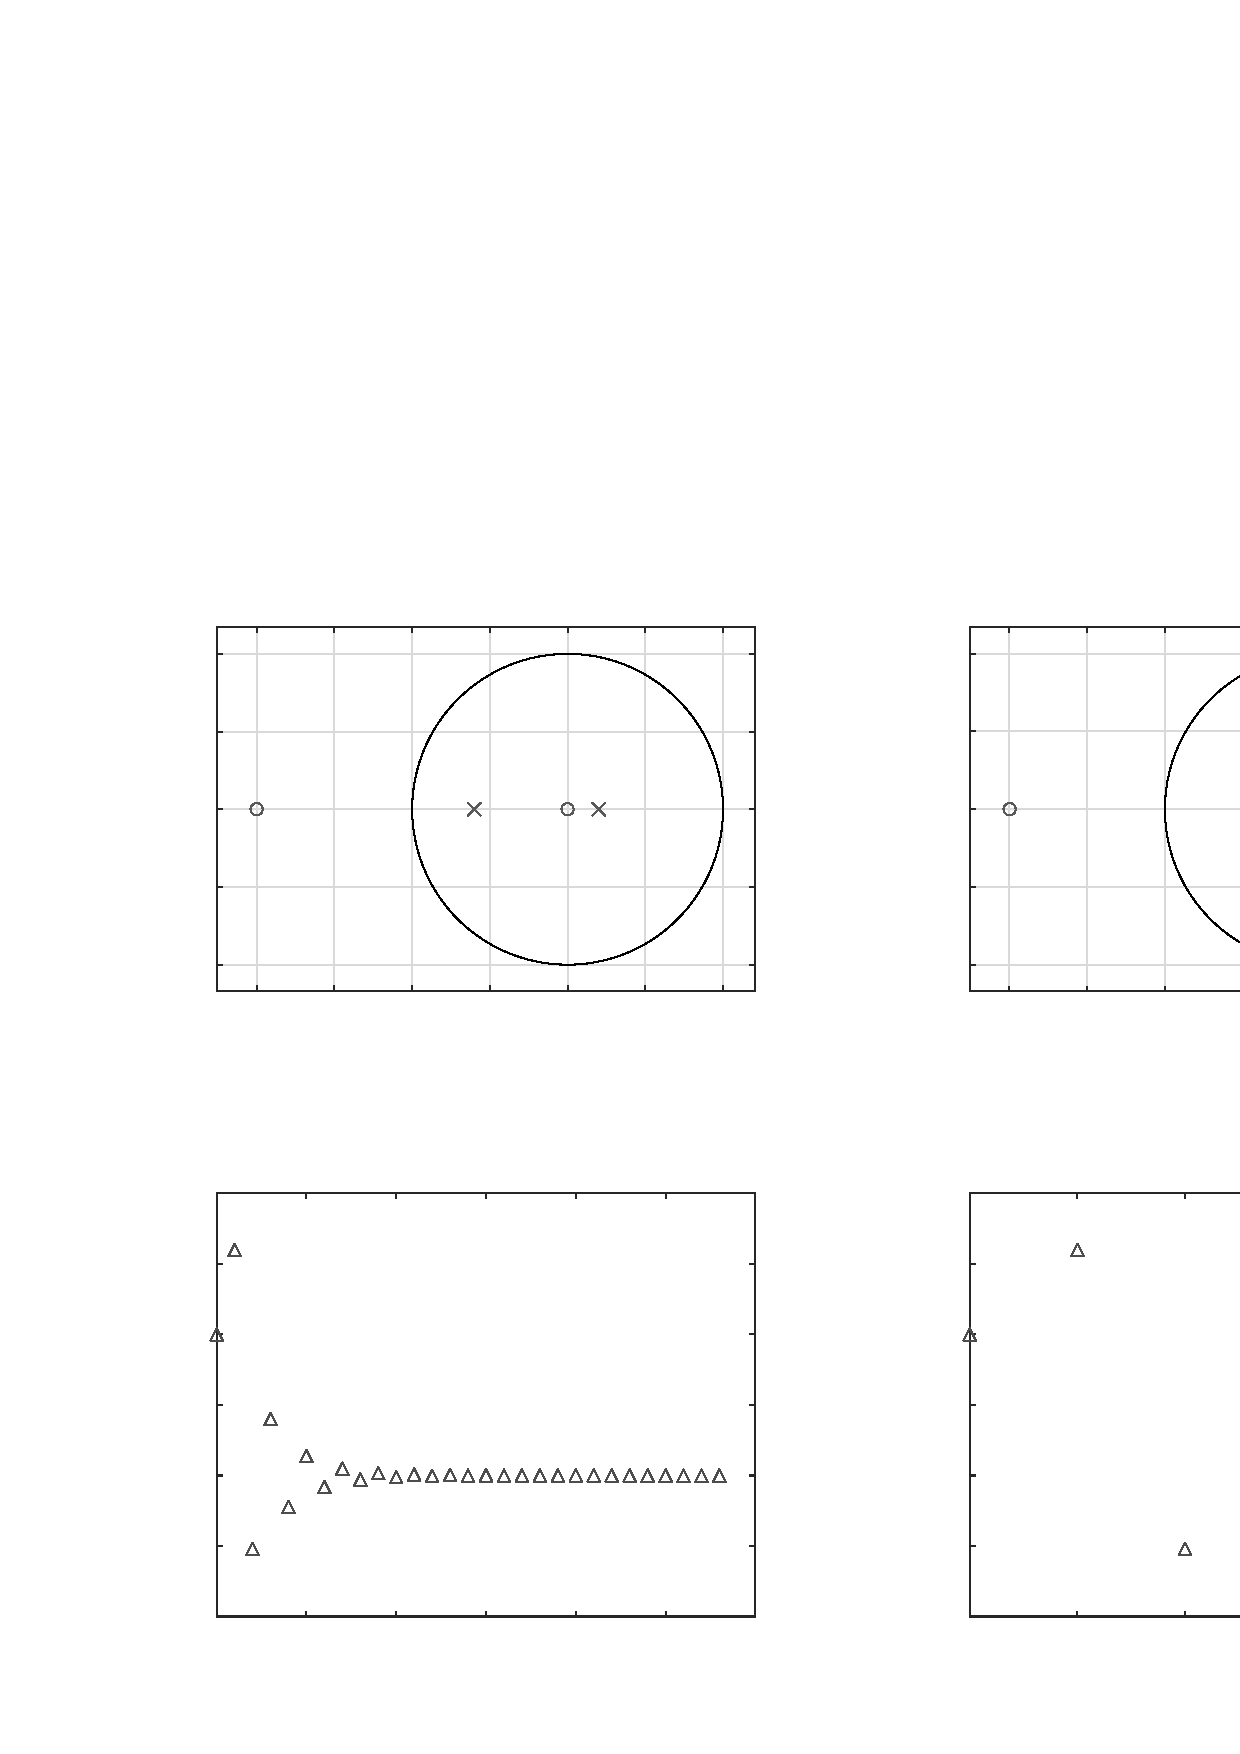
\includegraphics[scale=1]{octaves/zTransform1-inc}
\end{picture}%
\begin{picture}(800,600)(0,0)
\fontsize{13}{0}\selectfont\put(123.215,355.725){\makebox(0,0)[t]{\textcolor[rgb]{0.15,0.15,0.15}{{-2}}}}
\fontsize{13}{0}\selectfont\put(160.524,355.725){\makebox(0,0)[t]{\textcolor[rgb]{0.15,0.15,0.15}{{-1.5}}}}
\fontsize{13}{0}\selectfont\put(197.834,355.725){\makebox(0,0)[t]{\textcolor[rgb]{0.15,0.15,0.15}{{-1}}}}
\fontsize{13}{0}\selectfont\put(235.144,355.725){\makebox(0,0)[t]{\textcolor[rgb]{0.15,0.15,0.15}{{-0.5}}}}
\fontsize{13}{0}\selectfont\put(272.453,355.725){\makebox(0,0)[t]{\textcolor[rgb]{0.15,0.15,0.15}{{0}}}}
\fontsize{13}{0}\selectfont\put(309.763,355.725){\makebox(0,0)[t]{\textcolor[rgb]{0.15,0.15,0.15}{{0.5}}}}
\fontsize{13}{0}\selectfont\put(347.073,355.725){\makebox(0,0)[t]{\textcolor[rgb]{0.15,0.15,0.15}{{1}}}}
\fontsize{13}{0}\selectfont\put(97.0766,378.852){\makebox(0,0)[r]{\textcolor[rgb]{0.15,0.15,0.15}{{-1}}}}
\fontsize{13}{0}\selectfont\put(97.0766,416.162){\makebox(0,0)[r]{\textcolor[rgb]{0.15,0.15,0.15}{{-0.5}}}}
\fontsize{13}{0}\selectfont\put(97.0766,453.472){\makebox(0,0)[r]{\textcolor[rgb]{0.15,0.15,0.15}{{0}}}}
\fontsize{13}{0}\selectfont\put(97.0766,490.782){\makebox(0,0)[r]{\textcolor[rgb]{0.15,0.15,0.15}{{0.5}}}}
\fontsize{13}{0}\selectfont\put(97.0766,528.091){\makebox(0,0)[r]{\textcolor[rgb]{0.15,0.15,0.15}{{1}}}}
\fontsize{13}{0}\selectfont\put(484.444,355.659){\makebox(0,0)[t]{\textcolor[rgb]{0.15,0.15,0.15}{{-2}}}}
\fontsize{13}{0}\selectfont\put(521.789,355.659){\makebox(0,0)[t]{\textcolor[rgb]{0.15,0.15,0.15}{{-1.5}}}}
\fontsize{13}{0}\selectfont\put(559.133,355.659){\makebox(0,0)[t]{\textcolor[rgb]{0.15,0.15,0.15}{{-1}}}}
\fontsize{13}{0}\selectfont\put(596.478,355.659){\makebox(0,0)[t]{\textcolor[rgb]{0.15,0.15,0.15}{{-0.5}}}}
\fontsize{13}{0}\selectfont\put(633.823,355.659){\makebox(0,0)[t]{\textcolor[rgb]{0.15,0.15,0.15}{{0}}}}
\fontsize{13}{0}\selectfont\put(671.168,355.659){\makebox(0,0)[t]{\textcolor[rgb]{0.15,0.15,0.15}{{0.5}}}}
\fontsize{13}{0}\selectfont\put(708.513,355.659){\makebox(0,0)[t]{\textcolor[rgb]{0.15,0.15,0.15}{{1}}}}
\fontsize{13}{0}\selectfont\put(458.52,378.782){\makebox(0,0)[r]{\textcolor[rgb]{0.15,0.15,0.15}{{-1}}}}
\fontsize{13}{0}\selectfont\put(458.52,416.127){\makebox(0,0)[r]{\textcolor[rgb]{0.15,0.15,0.15}{{-0.5}}}}
\fontsize{13}{0}\selectfont\put(458.52,453.472){\makebox(0,0)[r]{\textcolor[rgb]{0.15,0.15,0.15}{{0}}}}
\fontsize{13}{0}\selectfont\put(458.52,490.817){\makebox(0,0)[r]{\textcolor[rgb]{0.15,0.15,0.15}{{0.5}}}}
\fontsize{13}{0}\selectfont\put(458.52,528.162){\makebox(0,0)[r]{\textcolor[rgb]{0.15,0.15,0.15}{{1}}}}
%\fontsize{13}{0}\selectfont\put(633.823,453.472){\makebox(0,0)[l]{\textcolor[rgb]{0.34524,0.34524,0.34524}{{ $^5$}}}}
\fontsize{13}{0}\selectfont\put(104,55.5941){\makebox(0,0)[t]{\textcolor[rgb]{0.15,0.15,0.15}{{0}}}}
\fontsize{13}{0}\selectfont\put(147.093,55.5941){\makebox(0,0)[t]{\textcolor[rgb]{0.15,0.15,0.15}{{5}}}}
\fontsize{13}{0}\selectfont\put(190.185,55.5941){\makebox(0,0)[t]{\textcolor[rgb]{0.15,0.15,0.15}{{10}}}}
\fontsize{13}{0}\selectfont\put(233.278,55.5941){\makebox(0,0)[t]{\textcolor[rgb]{0.15,0.15,0.15}{{15}}}}
\fontsize{13}{0}\selectfont\put(276.371,55.5941){\makebox(0,0)[t]{\textcolor[rgb]{0.15,0.15,0.15}{{20}}}}
\fontsize{13}{0}\selectfont\put(319.464,55.5941){\makebox(0,0)[t]{\textcolor[rgb]{0.15,0.15,0.15}{{25}}}}
\fontsize{13}{0}\selectfont\put(362.556,55.5941){\makebox(0,0)[t]{\textcolor[rgb]{0.15,0.15,0.15}{{30}}}}
\fontsize{13}{0}\selectfont\put(97.0766,66){\makebox(0,0)[r]{\textcolor[rgb]{0.15,0.15,0.15}{{-1}}}}
\fontsize{13}{0}\selectfont\put(97.0766,99.8427){\makebox(0,0)[r]{\textcolor[rgb]{0.15,0.15,0.15}{{-0.5}}}}
\fontsize{13}{0}\selectfont\put(97.0766,133.685){\makebox(0,0)[r]{\textcolor[rgb]{0.15,0.15,0.15}{{0}}}}
\fontsize{13}{0}\selectfont\put(97.0766,167.528){\makebox(0,0)[r]{\textcolor[rgb]{0.15,0.15,0.15}{{0.5}}}}
\fontsize{13}{0}\selectfont\put(97.0766,201.371){\makebox(0,0)[r]{\textcolor[rgb]{0.15,0.15,0.15}{{1}}}}
\fontsize{13}{0}\selectfont\put(97.0766,235.214){\makebox(0,0)[r]{\textcolor[rgb]{0.15,0.15,0.15}{{1.5}}}}
\fontsize{13}{0}\selectfont\put(97.0766,269.056){\makebox(0,0)[r]{\textcolor[rgb]{0.15,0.15,0.15}{{2}}}}
\fontsize{13}{0}\selectfont\put(465.444,55.5941){\makebox(0,0)[t]{\textcolor[rgb]{0.15,0.15,0.15}{{0}}}}
\fontsize{13}{0}\selectfont\put(517.155,55.5941){\makebox(0,0)[t]{\textcolor[rgb]{0.15,0.15,0.15}{{1}}}}
\fontsize{13}{0}\selectfont\put(568.866,55.5941){\makebox(0,0)[t]{\textcolor[rgb]{0.15,0.15,0.15}{{2}}}}
\fontsize{13}{0}\selectfont\put(620.577,55.5941){\makebox(0,0)[t]{\textcolor[rgb]{0.15,0.15,0.15}{{3}}}}
\fontsize{13}{0}\selectfont\put(672.289,55.5941){\makebox(0,0)[t]{\textcolor[rgb]{0.15,0.15,0.15}{{4}}}}
\fontsize{13}{0}\selectfont\put(724,55.5941){\makebox(0,0)[t]{\textcolor[rgb]{0.15,0.15,0.15}{{5}}}}
\fontsize{13}{0}\selectfont\put(458.52,66){\makebox(0,0)[r]{\textcolor[rgb]{0.15,0.15,0.15}{{-1}}}}
\fontsize{13}{0}\selectfont\put(458.52,99.8427){\makebox(0,0)[r]{\textcolor[rgb]{0.15,0.15,0.15}{{-0.5}}}}
\fontsize{13}{0}\selectfont\put(458.52,133.685){\makebox(0,0)[r]{\textcolor[rgb]{0.15,0.15,0.15}{{0}}}}
\fontsize{13}{0}\selectfont\put(458.52,167.528){\makebox(0,0)[r]{\textcolor[rgb]{0.15,0.15,0.15}{{0.5}}}}
\fontsize{13}{0}\selectfont\put(458.52,201.371){\makebox(0,0)[r]{\textcolor[rgb]{0.15,0.15,0.15}{{1}}}}
\fontsize{13}{0}\selectfont\put(458.52,235.214){\makebox(0,0)[r]{\textcolor[rgb]{0.15,0.15,0.15}{{1.5}}}}
\fontsize{13}{0}\selectfont\put(458.52,269.056){\makebox(0,0)[r]{\textcolor[rgb]{0.15,0.15,0.15}{{2}}}}
\end{picture}

    }\caption{Zeroes and poles of $G(z) = \frac{1 - 2z^{-1}}{1 + 0.4z^{-1} - 0.12z^{-2}}$ and of its FIR approximation (above), the related impulse responses (below). To obtain the length-$6$ FIR approximation from the numerator and the denominator of the $z$-transform, run \texttt{num2 = impz(num1,den1,6)', den2 = 1;} octave code. Complete code can be found in file \texttt{zTransform1.m}.}\label{oct:zTransform1}
\end{center}
\end{figure*}

\begin{figure*}[ht]
\begin{center}
\scalebox{0.4}{
% Title: gl2ps_renderer figure
% Creator: GL2PS 1.4.2, (C) 1999-2020 C. Geuzaine
% For: Octave
% CreationDate: Wed Nov  2 14:36:59 2022
\setlength{\unitlength}{1pt}
\begin{picture}(0,0)
\includegraphics[scale=1]{octaves/zTransform2-inc}
\end{picture}%
\begin{picture}(800,600)(0,0)
\fontsize{13}{0}\selectfont\put(373.458,148.96){\makebox(0,0)[tl]{\textcolor[rgb]{0.15,0.15,0.15}{{2}}}}
\fontsize{13}{0}\selectfont\put(314.939,110.968){\makebox(0,0)[tl]{\textcolor[rgb]{0.15,0.15,0.15}{{0}}}}
\fontsize{13}{0}\selectfont\put(344.198,129.964){\makebox(0,0)[tl]{\textcolor[rgb]{0.15,0.15,0.15}{{1}}}}
\fontsize{13}{0}\selectfont\put(93.0986,228.825){\makebox(0,0)[br]{\textcolor[rgb]{0.15,0.15,0.15}{{-4}}}}
\fontsize{13}{0}\selectfont\put(146.501,119.043){\makebox(0,0)[tr]{\textcolor[rgb]{0.15,0.15,0.15}{{0}}}}
\fontsize{13}{0}\selectfont\put(127.791,139.673){\makebox(0,0)[tr]{\textcolor[rgb]{0.15,0.15,0.15}{{0.5}}}}
\fontsize{13}{0}\selectfont\put(109.081,160.303){\makebox(0,0)[tr]{\textcolor[rgb]{0.15,0.15,0.15}{{1}}}}
\fontsize{13}{0}\selectfont\put(90.3716,180.933){\makebox(0,0)[tr]{\textcolor[rgb]{0.15,0.15,0.15}{{1.5}}}}
\fontsize{13}{0}\selectfont\put(165.211,98.4124){\makebox(0,0)[tr]{\textcolor[rgb]{0.15,0.15,0.15}{{-0.5}}}}
\fontsize{13}{0}\selectfont\put(183.92,77.7823){\makebox(0,0)[tr]{\textcolor[rgb]{0.15,0.15,0.15}{{-1}}}}
\fontsize{13}{0}\selectfont\put(202.63,57.1521){\makebox(0,0)[tr]{\textcolor[rgb]{0.15,0.15,0.15}{{-1.5}}}}
\fontsize{13}{0}\selectfont\put(227.16,53.9797){\makebox(0,0)[tl]{\textcolor[rgb]{0.15,0.15,0.15}{{-3}}}}
\fontsize{13}{0}\selectfont\put(256.419,72.9758){\makebox(0,0)[tl]{\textcolor[rgb]{0.15,0.15,0.15}{{-2}}}}
\fontsize{13}{0}\selectfont\put(285.679,91.9719){\makebox(0,0)[tl]{\textcolor[rgb]{0.15,0.15,0.15}{{-1}}}}
\fontsize{13}{0}\selectfont\put(93.0986,282.873){\makebox(0,0)[br]{\textcolor[rgb]{0.15,0.15,0.15}{{-2}}}}
\fontsize{13}{0}\selectfont\put(93.0986,336.921){\makebox(0,0)[br]{\textcolor[rgb]{0.15,0.15,0.15}{{0}}}}
\fontsize{13}{0}\selectfont\put(93.0986,390.968){\makebox(0,0)[br]{\textcolor[rgb]{0.15,0.15,0.15}{{2}}}}
\fontsize{13}{0}\selectfont\put(93.0986,445.016){\makebox(0,0)[br]{\textcolor[rgb]{0.15,0.15,0.15}{{4}}}}
\fontsize{13}{0}\selectfont\put(705.642,129.964){\makebox(0,0)[tl]{\textcolor[rgb]{0.15,0.15,0.15}{{1}}}}
\fontsize{13}{0}\selectfont\put(454.542,228.825){\makebox(0,0)[br]{\textcolor[rgb]{0.15,0.15,0.15}{{-4}}}}
\fontsize{13}{0}\selectfont\put(676.382,110.968){\makebox(0,0)[tl]{\textcolor[rgb]{0.15,0.15,0.15}{{0}}}}
\fontsize{13}{0}\selectfont\put(451.815,180.933){\makebox(0,0)[tr]{\textcolor[rgb]{0.15,0.15,0.15}{{1.5}}}}
\fontsize{13}{0}\selectfont\put(470.525,160.303){\makebox(0,0)[tr]{\textcolor[rgb]{0.15,0.15,0.15}{{1}}}}
\fontsize{13}{0}\selectfont\put(489.235,139.673){\makebox(0,0)[tr]{\textcolor[rgb]{0.15,0.15,0.15}{{0.5}}}}
\fontsize{13}{0}\selectfont\put(507.944,119.043){\makebox(0,0)[tr]{\textcolor[rgb]{0.15,0.15,0.15}{{0}}}}
\fontsize{13}{0}\selectfont\put(526.654,98.4124){\makebox(0,0)[tr]{\textcolor[rgb]{0.15,0.15,0.15}{{-0.5}}}}
\fontsize{13}{0}\selectfont\put(545.364,77.7823){\makebox(0,0)[tr]{\textcolor[rgb]{0.15,0.15,0.15}{{-1}}}}
\fontsize{13}{0}\selectfont\put(564.074,57.1521){\makebox(0,0)[tr]{\textcolor[rgb]{0.15,0.15,0.15}{{-1.5}}}}
\fontsize{13}{0}\selectfont\put(588.603,53.9797){\makebox(0,0)[tl]{\textcolor[rgb]{0.15,0.15,0.15}{{-3}}}}
\fontsize{13}{0}\selectfont\put(617.863,72.9758){\makebox(0,0)[tl]{\textcolor[rgb]{0.15,0.15,0.15}{{-2}}}}
\fontsize{13}{0}\selectfont\put(647.123,91.9719){\makebox(0,0)[tl]{\textcolor[rgb]{0.15,0.15,0.15}{{-1}}}}
\fontsize{13}{0}\selectfont\put(734.901,148.96){\makebox(0,0)[tl]{\textcolor[rgb]{0.15,0.15,0.15}{{2}}}}
\fontsize{13}{0}\selectfont\put(454.542,282.873){\makebox(0,0)[br]{\textcolor[rgb]{0.15,0.15,0.15}{{-2}}}}
\fontsize{13}{0}\selectfont\put(454.542,336.921){\makebox(0,0)[br]{\textcolor[rgb]{0.15,0.15,0.15}{{0}}}}
\fontsize{13}{0}\selectfont\put(454.542,390.968){\makebox(0,0)[br]{\textcolor[rgb]{0.15,0.15,0.15}{{2}}}}
\fontsize{13}{0}\selectfont\put(454.542,445.016){\makebox(0,0)[br]{\textcolor[rgb]{0.15,0.15,0.15}{{4}}}}
\end{picture}

    }\caption{Plot of $G(z) = \frac{1 - 2z^{-1}}{1 + 0.4z^{-1} - 0.12z^{-2}}$ (left) and of its FIR approximation (right). Notice the correspondence between these two plots and the location of zeros and poles in Figure~\ref{oct:zTransform1}.}\label{oct:zTransform2}
\end{center}
\end{figure*}

